%
%   CHAPTER : HOW WEHRE EXPERIMENTS CONDUCTED
%   
%   Wichtige Punkte : 
%    + verallgemeinerung der müller-matrix über integration
%    + bauteil charakterisierung -> berechnung der Müllermatrix für Fasern
%    + simulation von Tetra, Phenylalanin
%    + Weißlichtspektren
%    + sample spectra
%
\documentclass[a4paper,12pt,twoside,parskip=no,headsepline,open=right,ngerman,export]{scrreprt}

%
%   Include shared preamble
%   Preamble is put into seperate file to be used in files included with \input
%   Made possible with standalone package
%
%
%   PREAMBLE SHARED BY MASTER FILE AND ALL SUBFILES
%
%
%   USED PACKAGES AND STYLES
%

%
%   KEINE AHNUNG; IST KRAM DEN JULIAN IN SEINEM TEMPLATE HATTE
%
\usepackage{newunicodechar}
\usepackage{comment}
%\usepackage{acro} %Abkürzungen
\usepackage{xcolor} %Farben
\usepackage{rotating}
\usepackage{lmodern}
%\usepackage{parskip}
%\usepackage[crop=off]{auto-pst-pdf} %Einbinden von .eps-Dateien in PDFTeX
\usepackage{paralist}

%
%   UTILITIES
%
%\usepackage{hyperref}

%
%   LANGUAGE, FONT
%
\usepackage[utf8]{inputenc} % Eingabe-Codierung
\usepackage[ngerman]{babel} % Spracheinstellung
\usepackage[T1]{fontenc}    % Anpassung auf europäischen Zeichensatz
\usepackage{xspace}         % Leerzeichen für Silbentrennung
\usepackage{hyphenat}       % Korrekte Silbentrennung


%
%   MULTIPLE FILES
%
\usepackage{pdfpages}   % Include pdf files
\usepackage{standalone} % Include .tex/.Rtex documents that have their own preamble and \begin{documents}

%
%   INHALTSVERZEICHNIS UND ÄHNLICHES
%
%%Umbennenung Inhaltsverzeichnis
\addto\captionsenglish{%
\renewcommand{\contentsname}{Inhaltsverzeichnis}}

%
%   FIGURES AND TABLES
%
\usepackage{subfig}                     % Mutli image figures
\usepackage[format=plain]{caption} %Einstellen der caption-Breite
\captionsetup[table]{skip=10pt}
\usepackage{wrapfig} %Floats von Text umflossen
\usepackage{float} %Position von figure/table erzwingen
\usepackage{flafter} %Floats nach Definition!
\usepackage{graphicx}
\usepackage{booktabs}
\usepackage{multicol}
\usepackage{multirow}


%
%   LITERATUR
%
\usepackage[style=chem-angew,
            doi=true,
			sorting=none,
			backend=biber,
			autocite=superscript,    % Zitate
			minbibnames=3,
			maxbibnames=5
			]{biblatex}
\usepackage{csquotes}                % Formattieren von Zitaten (Anfürhungszeichen)


%
%   MATHEMATIK
%
\usepackage{amsmath} %mathematischer Satz
\usepackage{amsfonts} %mathematische Schriftart
\usepackage{amssymb} %mathematische Symbole
\usepackage[output-decimal-marker={,},
            group-separator = {.}, 
            group-digits=true,
            detect-weight]{siunitx}     % korrekte Formatierung von Einheiten nach SI-Kriterien
\usepackage{nicefrac}
\usepackage{mathtools}  % pmatrix* environment for aligning matrix elements

%
%   CHEMIE
%
%\usepackage{chemgreek}
%\usepackage{chemnum} %Nummerierung der Verbindung aus ChemDraw
\usepackage[version=4]{mhchem} %Darstellung von chemischen Formeln
\usepackage{chemmacros}         % Abkürzungen (pH, pKa, ...) und Ladungen

%
%   FORMATTING, PAGE STYLE
%
\usepackage{setspace} %Zeilenabstand
%\usepackage{titlesec} %Verändern von Überschrift-Formatierungen
\usepackage[headsepline]{scrlayer-scrpage}

%
% INCLUDE SOURCE CODE
%
\definecolor{dkgreen}{rgb}{0,0.6,0}
\definecolor{gray}{rgb}{0.5,0.5,0.5}
\definecolor{mauve}{rgb}{0.58,0,0.82}
\usepackage{listings} %Programmiersprachen einbinden
\lstloadlanguages{R}
\lstset{frame=tb,
  language=R,
  aboveskip=3mm,
  belowskip=3mm,
  showstringspaces=false,
  columns=flexible,
  basicstyle={\small\ttfamily},
  numbers=none,
  numberstyle=\tiny\color{gray},
  keywordstyle=\color{blue},
  commentstyle=\color{dkgreen},
  stringstyle=\color{mauve},
  breaklines=true,
  breakatwhitespace=true,
  tabsize=4
}



%
%   JULIANS TEMPLATE COMMANDS
%   KEINE AHNUNG WAS ER DA GEMACHT HAT
%
\newcommand{\ts}{\textsubscript} %tiefstellen
\newcommand{\te}{\textsuperscript} %hochstellen
\newcommand{\grad}{\degreeCelsius}


%\setlength{\parindent}{0pt}


\setcounter{secnumdepth}{4}

\DeclareUnicodeCharacter{00A0}{ }

\newlength\myheight

\newlength\mywidth



\clubpenalty10000
\widowpenalty10000
\displaywidowpenalty=10000

%\raggedbottom

%\renewcommand{\lstlistingname}{Code}

\floatstyle{plaintop}
\newfloat{code}{tbp}{lop}[chapter]
\floatname{code}{Code}
%
%   ENDE JULIANS TEMPLATE
%	
%
%   SOME CUSTOM COMMANDS AND SHORTCUTS
%

% MATHEMATICS AND FORMULAS
\newcommand{\ring}[1]{\text{\r{#1}}}	    % Shortcut for writing circle above character
\newcommand{\vc}[1]{\vec{#1}}               % Shortcut for uniformly formatting vectors
\newcommand{\mx}[1]{\boldsymbol#1}          % Shrotcut for uniformly formatting matrices
\newcommand{\tildenu}{\tilde{\nu}}          % Shortcut for wave number symbol

% FORMATTING
\newcommand{\optelem}[1]{\textbf{#1}}       % Shortcut for uniforly formate optical elements
\newcommand{\chemical}[1]{\textbf{#1}}      % Shortcut for uniforly formate chemical abreviations

% REMINDERS
\def\quelle{~\textbf{[QUELLE]}}

% -----------------------------------------
% Makros used to make integral sign match matrix/fraction height
%
\def\tmp#1 #2\relax{#1}
\setbox0=\hbox{$\xdef\intfont{%
    \expandafter\tmp\fontname\textfont3\expandafter\space\space\relax}$}
\font\tmp=\intfont\space at10pt\relax
\setbox0=\hbox{$\textfont3=\tmp \displaystyle \int$}
\dimen0=\ht0 \advance\dimen0 by\dp0 \divide\dimen0 by10 
\xdef\intsize{\the\dimen0}

\def\dividedimen (#1/#2){\expandafter\ignorept\the
   \dimexpr\numexpr\number\dimexpr#1\relax
   *65536/\number\dimexpr#2\relax\relax sp\relax
}
{\lccode`\?=`\p \lccode`\!=`\t  \lowercase{\gdef\ignorept#1?!{#1}}}
% Makros used to make integral sign match matrix/fraction height
\def\flexibleint{\def\fxintL{}\def\fxintU{}\futurelet\next\fxintA}
\def\fxintA{\ifx\next_\expandafter\fxintB\else\expandafter\fxintC\fi}
\def\fxintB_#1{\def\fxintL{#1}\fxintC}
\def\fxintC{\futurelet\next\fxintD}
\def\fxintD{\ifx\next^\expandafter\fxintE\else\expandafter\fxintF\fi}
\def\fxintE^#1{\def\fxintU{#1}\fxintF}
\def\fxintF#1{\begingroup
   \setbox0=\hbox{$\displaystyle{#1}$}%
   \dimen0=\ht0 \advance\dimen0 by\dp0
   \setbox1=\hbox{$\vcenter{\copy0}$}%
   \font\tmp=\intfont\space at\dividedimen(\dimen0/\intsize)pt
   \lower\dimexpr\dp0-\dp1\hbox{%
      $\textfont3=\tmp \displaystyle\int_{\fxintL}^{\fxintU}$}
   \box0
   \endgroup
}
%
% END: makros for making integral match fraction/matrix height
% --------------------------------------------
%\input{./sup/abreviations.tex}
%
%   CUSTOM HYPHENATION
%

%\hyphenation{Kor-re-la-ti-ons-spek-tro-sko-pie Kor-re-la-ti-ons-spek-trum Spek-tro-sko-pie}
\hyphenation{Stan-dard-ab-wei-chung}
\hyphenation{Halb-wel-len-plat-te Halb-wel-len-plat-ten}
\hyphenation{Ra-man-Mül-ler-trans-for-ma-tion}
\hyphenation{An-ti-Sto-kes-Ver-schie-bung}
\hyphenation{Sto-kes-Ver-schie-bung}


%
%   LITERATUR
%
\addbibresource{./sup/lit.bib}	
\AtEveryBibitem{\clearfield{note}}    % clears notes

%
%   SEITENEINSTELLUNG
%
%Druckbereich wählen (\areaset[BCOR]{breite}{höhe})
\areaset[13 mm]{140mm}{250mm}
\pagestyle{scrheadings}


%
%   KOPFZEILE
%
\chead{\leftmark}
\ihead{}
\ohead{}
\ofoot{\thepage}
\automark{chapter}


%
%   SEITENSTIL
%
\setstretch{1.15} %Zeilenabstand einstellen
\pagenumbering{arabic}
\setcounter{page}{1}

%
%   DOCUMENT
%
\begin{document}
    
    \chapter{Methodik}
    
        Im Zuge dieser Arbeit wurden Ramanspektren in Abhängigkeit der Polarisations des anregenden Lasers gemessen. Vorbereitend wurden weitere Experimente zur Charakterisierung der verwendeten Bauteile durchgeführt. Tabelle~\ref{tab:mehtod_equippment} listet die genutzten Geräte und Bauteile auf. Zusätzlich wurde das Ramanspektrometer folgenden Spezifikationen eingesetzt. Das Ramanspektrometer wird in Zukunft mit WiTec abgekürzt. In allen Experimenten wurde der Anregungslaser des WiTecs als Strahlungsquelle verwendet.
        
        WiTec alpha300, ZaF: Raman-Mikroskop (WiTec GmbH, Ulm). Objektiv: EC Epiplan DIC, 10x, $N\!A = \num{0.25}$ (Carl Zeiss AG, Oberkochen). Anregungsquelle: Dioden-gepumpter Festkörperlaser (Cobolt, Solna, Schweden), \SI{514}{nm}. Detektor: Thermoelektrisch gekühlte CCD (\SI{-70}{\degree}). Gitter: \SI{600}{g/mm} $\mathit{BLZ}=\SI{500}{nm}$.
        
        Die Fiberbenches koppelten Licht aus einer Faser aus und koppelten es nach wenigen Zentimetern in eine zweite Faser wieder ein. Dadurch konnten verschiedene optische Elemente im Strahlengang platziert werden, um die Polarisation der Strahlung zu beeinflussen. Die folgenden Abschnitte beschreiben die durchgeführten Experimente.
        
        \begin{table}[!h]
            \centering
            \caption[Liste genutzter Geräte und ihre Kürzel]{Liste genutzter Geräte mit ihrer Bezeichnung und Kürzel.}
            \label{tab:mehtod_equippment}
            \begin{tabular}{lll}
                \toprule
                Kürzel          & Bauteil           & Bezeichnung               \\
                \midrule
                \optelem{PM}    & Powermeter        & ThorLabs PM100D/S130C     \\ 
                \optelem{P1}    & Linearpolarisator & ThorLabs FBR-LPVIS        \\ 
                \optelem{P2}    & Linearpolarisator & ThorLabs FBR-LPVIS        \\
                \optelem{P3}    & Linearpolarisator & ThorLabs LPVISA050-MP2    \\
                \optelem{P4}    & Linearpolarisator & ThorLabs LPVISA050-MP2    \\
                \optelem{DP}    & Depolarisator     & ThorLabs DPP25-A          \\
                \optelem{B1}    & Fiberbench        & ThorLabs FBP-A-FC         \\
                \optelem{B2}    & Fiberbench        & ThorLabs FBP-A-FC         \\
                \optelem{F1}    & PM-Faser          & ThorLabs P1-488PM-FC-1    \\
                \optelem{F2}    & SM-Faser          & ThorLabs P1-460B-FC-1     \\
                \optelem{F3}    & MM-Faser          & ThorLabs M122L01          \\
                \optelem{W1}    & Halbwellenplatte  & ThorLabs FBR-AH1          \\
                \optelem{W2}    & Halbwellenplatte  & ThorLabs FBR-AH1          \\
                \bottomrule
            \end{tabular}
        \end{table}
        
        \section{Charakterisierung optischer Bauteile}\label{sec:appendix_method_characterisation}
            
            Charakterisiert wurden die Linearpolarisatoren aus Natriumsilikat \optelem{P1} und \optelem{P2}, der Linearpolarisator mit Nanopartikelbeschichtung \optelem{P3}, die Halbwellenplatten \optelem{W1} und \optelem{W2} sowie die polarisationserhaltene Faser \optelem{F1}, single-mode Faser \optelem{F2} und multi-mode Faser \optelem{F3}.



            \subsection*{Linearpolarisatoren}
            
            Für die Linearpolarisatoren \optelem{P1}, \optelem{P2} und \optelem{P3} wurde geprüft, ob das Transmissionsverhalten der Polarisatoren abhängig von Ihrer Orientierung ist, wenn die Polarisationsebene des Lasers parallel zu Ihnen ausgerichtet bleibt. Zusätzlich wurde mit \optelem{P1} und \optelem{P2} der Transmissionsgrad von Polarisatoren in Abhängigkeit ihrer Rotation gegen die Polarisationsebene des Lasers gemessen.
            
            \begin{figure}[!b]
                %
                %   Aufbau: Transmissionsverhalten Linearpolarisator
                %
                \centering
                \subfloat[]{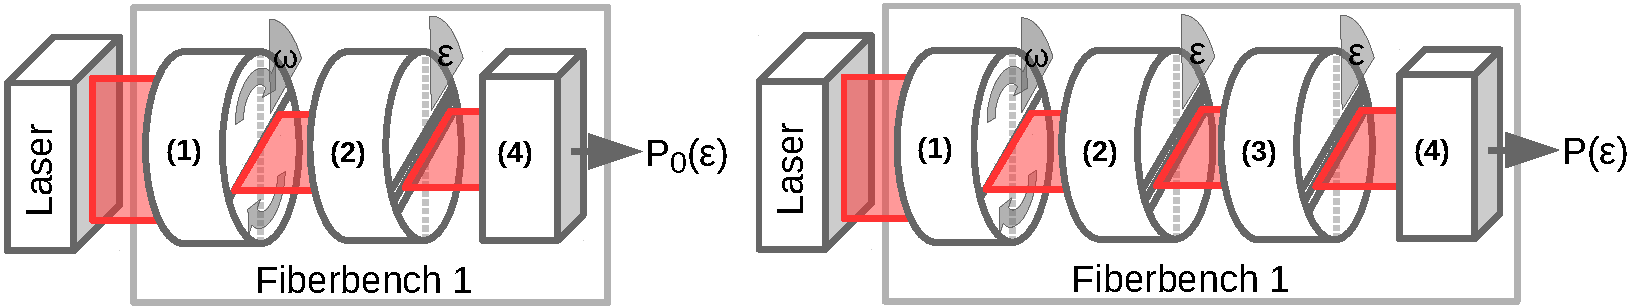
\includegraphics[width=\textwidth]{img/aufbau_linearpolarisator_transmission-A.pdf}\label{subfig:method_transmissionPolarisator-P1}}
                \\
                \subfloat[]{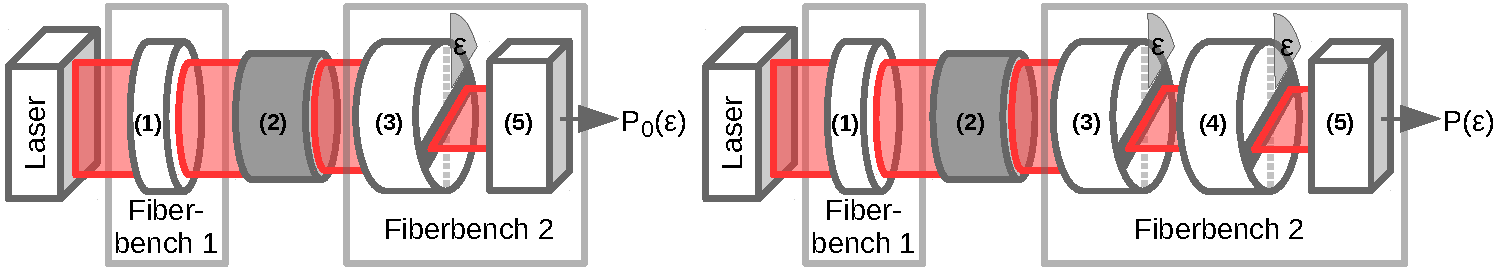
\includegraphics[width=\textwidth]{img/aufbau_linearpolarisator_transmission-B.pdf}\label{subfig:method_transmissionPolarisator-P3}}
                \caption[Transmissionsgrad von parallel polarisierten Licht]{Der experimentelle Aufbau zur Messung des Transmissionsverhaltens von parallel polarisierter Strahlung. 
                Der Aufbau~\subref{subfig:method_transmissionPolarisator-P1} wurde für \optelem{P1} und \optelem{P2} verwendet: Die Halbwellenplatte (1) wurde um beliebige Winkel $\omega$ gedreht, der auxilliare Linearpolarisator (2) und der charakterisierte Linearpolarisator (3) wurden parallel zu (1) orientiert. Nachdem (1) die Polarisationsebene des Lasers gedreht hatte, garantierte (2) vollständig polarisierte Strahlung. Das Powermeter (4) maß die Leistung des Lasers $P$. 
                Der Aufbau \subref{subfig:method_transmissionPolarisator-P3} wurde für \optelem{P3} verwendet: Der Laserstrahl wurde durch den Depolarisator (1) und eine optische Faser (2) depolarisiert. Der auxilliare Linearpolarisator (3) polarisierte die Lichtwelle entlang eines beliebigen Winkels $\varepsilon$ parallel zum charakterisierten Polarisator (4). Das Powermeter (5) maß die Leistung $P$.}
                \label{fig:method_transmissionPolarisator}
            \end{figure}
            \begin{figure}[!b]
                %
                %   Aufbau: Polarisationsverhalten Linearpolarisator
                %
                \centering
                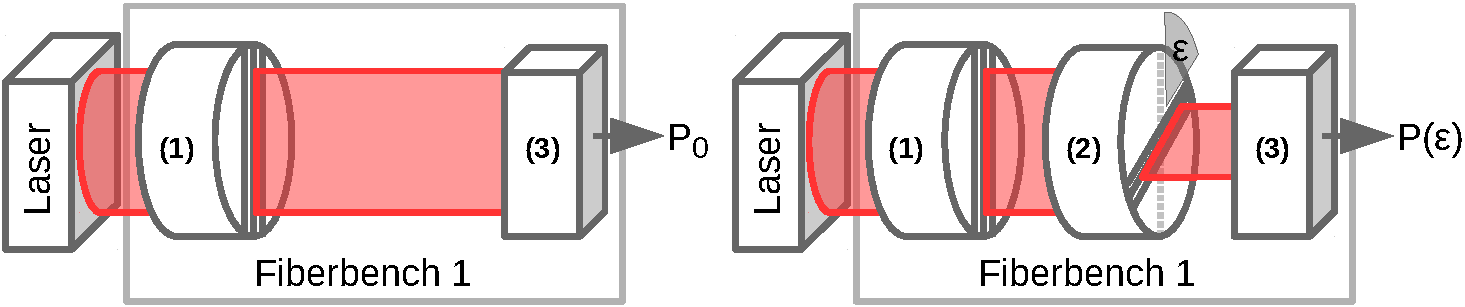
\includegraphics[width=\textwidth]{img/aufbau_linearpolarisator_polarisation.pdf}
                \caption[Polarisationsverhalten von Linearpolarisatoren]{Der experimentelle Aufbau zur Messung des Polarisationsverhaltens von \optelem{P1} und \optelem{P2}. Der auxilliare Polarisator~(1) polarisierte die Strahlung in 0°-Richtung. Der charakterisierte Polarisator~(2) wurde um beliebige Winkel $\varepsilon$ gedreht und die Leitung am Powermeter~(3) in Abhängigkeit von $\varepsilon$ gemessen.}
                \label{fig:method_polarisationPolarisator}
            \end{figure}
            
            Weil der Linearpolarisator \optelem{P3} länger als \optelem{P1} und \optelem{P2} ist, konnte der Aufbau~\ref{subfig:method_transmissionPolarisator-P1} aus Platzgründen nicht verwendet werden. Die Untersuchung des Transmissionsverhaltens von \optelem{P1} und \optelem{P2} mit dem Aufbau \ref{subfig:method_transmissionPolarisator-P1} erfolgte für beliebige Rotationen der Halbwellenplatte \optelem{W1}. Der auxilliare und der zu charakterisierende Linearpolarisator \optelem{P1} und \optelem{P2} wurden so gegen \optelem{W1} gedreht, dass die vom Powermeter gemessene Laserleistung maximal wurde. Es wurde festgehalten: Der Rotationswinkel der Halbwellenplatte, die Rotationswinkel beider Linearpolarisatoren und die Laserleistung gemessen vor und hinter dem zu charakterisierenden Linearpolarisator.
            
            Das Transmissionsverhalten von \optelem{P3} wurde mit Aufbau~\ref{subfig:method_transmissionPolarisator-P3} charakterisiert. Anstelle einer Halbwellenplatte wurde die Variation der Laserpolarisation durch einen Depolarisator, eine stark depolarisierende optische Faser und einen Linearpolarisator erreicht. Von dem Depolarisator und der depolarisierenden Faser wird folgend nur als Depolarisator gesprochen. Der depolarisierte Laserstrahl wurde durch den auxilliaren Linearpolarisator \optelem{P4} entlang einer beliebigen Polarisationsebene repolarisiert. Der zu charakterisierende Linearpolarisator \optelem{P3} wurde so gedreht, dass die vom Powermeter gemessene Laserleistung maximal wurde. Es wurde festgehalten: Der Rotationswinkel der beiden Linearpolarisatoren sowie die Laserleistung vor und hinter \optelem{P3}.
            
            Abbildung~\ref{fig:method_polarisationPolarisator} zeigt den Aufbau zur Bestimmung der Polarisationseigenschaften von \optelem{P1} und \optelem{P2}. Der auxilliare Linearpolarisator wurde so gegen den Laserstrahl verdreht, dass die transmittierte Laserleistung maximal wurde. Wenn \optelem{P1} charakterisiert wurde, war \optelem{P2} der auxilliare Linearpolarisator. Wurde \optelem{P2} charakterisiert, war \optelem{P1} der auxilliare Polarisator. Anschließend wurde der zu charakterisierende Polarisator dem Aufbau hinzugefügt und um beliebige Winkel rotiert. Für jeden Rotationswinkel des Polarisators wurde die Laserleistung vor und hinter dem zu charakterisierenden Polarisator gemessen. Es wurde festgehalten: Die Laserleistung gemessen vor und hinter dem charakterisierten Polarisator und sein Rotationswinkel.
            
            
            
            \subsection*{Halbwellenplatten}
            
            \begin{figure}[!b]
                \centering
                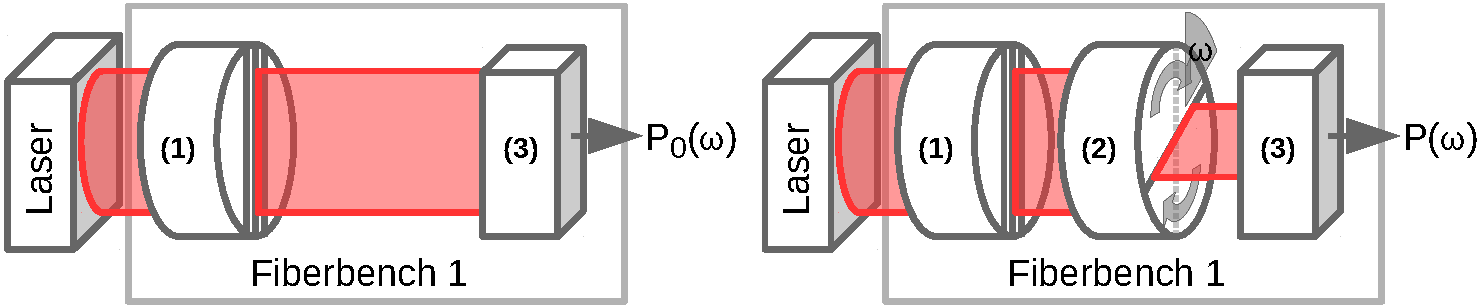
\includegraphics[width=\textwidth]{img/aufbau_wellenplatte_transmission.pdf}
                \caption[Bestimmung des Transmissionsverhaltens von Halbwellenplatten]{Der experimentelle Aufbau zur Bestimmung des Transmissionsverhaltens von \optelem{W1} und \optelem{W2} in Abhängigkeit der Polarisation der einfallenden Lichtwelle. Der Laserstrahl wurde durch Polarisator (1) entlang einer konstanten Achse linear polarisiert. Die Wellenplatte (2) wurde um beliebige Winkel $\omega$ gegen die Polarisationsebene rotiert. das Powermeter (3) maß die Leistung $P$.}
                \label{fig:method_transmissionWellenplatte}
            \end{figure}            
            
            Analog zu den Linearpolarisatoren wurden die Halbwellenplatten \optelem{W1} und \optelem{W2} hinsichtlich ihres Transmissionsverhaltens für verschieden linear polarisierte Strahlung und ihren Einfluss auf die Polarisation von Lichtwellen charakterisiert.
            
            Das Transmissionsverhalten wurde mit dem Aufbau in Abbildung~\ref{fig:method_transmissionWellenplatte} bestimmt. Dafür wurde der Linearpolarisator \optelem{P1} in den Strahlengang gestellt und so orientiert, dass die messbare Leistung hinter \optelem{P1} maximal war. Anschließend wurde die zu charakterisierende Halbwellenplatte in den Strahlengang gestellt und die Leistung vor und hinter der Halbwellenplatte mit dem Powermeter gemessen. Die Messung wurde für beliebige Rotationen der Halbwellenplatte wiederholt. Es wurde festgehalten: Die Position der Halbwellenplatte sowie die Laserleistung vor und hinter der Halbwellenplatte.
            
            \begin{figure}[!b]
                \centering
                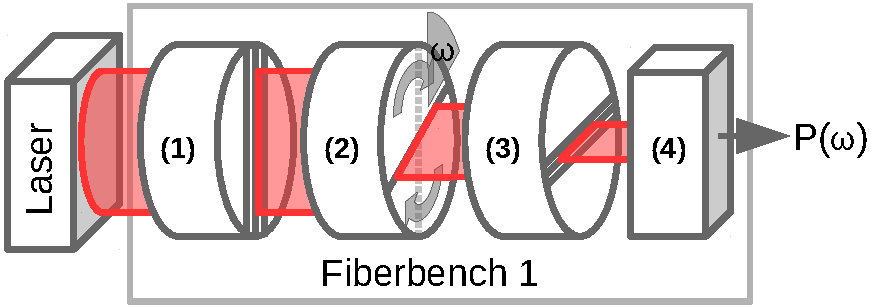
\includegraphics[width=0.6\textwidth]{img/aufbau_wellenplatte_rotation.pdf}
                \caption[Bestimmung des Einflusses von Halbwellenplatten auf Lichtwellen]{Der experimentelle Aufbau zur Bestimmung des Einflusses von Halbwellenplatten auf linear polarisierte Strahlung. Der Linearpolarisator (1) war parallel zum Laser ausgerichtet und sorgte für einen maximalen Polarisationsgrad, bevor die Polarisationsebene durch die Halbwellenplatte (2) gedreht wurde. Die Wellenplatte wurde um beliebige Winkel $\omega$ gegen (1) verdreht. Der Linearpolarisator (3) war orthogonal zu (1) orientiert und das Powermeter (4) maß die Laserleistung $P(\omega)$.}
                \label{fig:method_rotationWellenplatte}
            \end{figure}
            
            Für das zweite Experiment wurde der Aufbau aus Abbildung~\ref{fig:method_rotationWellenplatte} verwendet. Um den Einfluss einer Halbwellenplatte auf die Lage der Polarisationsebene einer linear polarisierten Lichtwelle zu charakterisieren, wurde Linearpolarisator \optelem{P1} im Strahlengang plaziert und so gedreht, dass die messbare Laserleistung hinter ihm maximal wurde. Anschließend wurde der zweite Linearpolarisator \optelem{P2} hinter \optelem{P1} in den Strahlengang gestellt und so gedreht, dass die messbare Laserleistung hinter ihm minimal wurde. Für die eigentliche Messung befand sich die zu charakterisierende Halbwellenplatte zwischen den Linearpolarisatoren. Für beliebige Rotationen der Halbwellenplatte wurde festgehalten: Der Rotationswinkel selbst und die hinter dem zweiten Linearpolarisator gemessene Laserleistung.
            
            
            
            \subsection*{Optische Fasern}\label{subsec:method_fibre}
            
            Die polarisationserhaltende Faser \optelem{F1}, Einmodenfaser \optelem{F2} und die Mehrmodenfaser \optelem{F3} wurden durch ihr Transmissionsverhalten in Abhängigkeit der Lichtpolarisation und die Bestimmung der Stokesvektoren vor und hinter der Faser charakterisiert. Es wurden nur die ersten drei Komponenten der Stokesvektoren ermittelt. Die zirkular polarisierte Komponente wurde vernachlässigt. Zusätzlich wurde der Einfluss von \optelem{F2} und \optelem{F3} auf die Lage der Polarisationsebene linear polarisierter Strahlung direkt bestimmt.
            
            \begin{figure}[!b]
                %
                %  MESSEN TRANSMISSION VON FASER
                %
                \center
                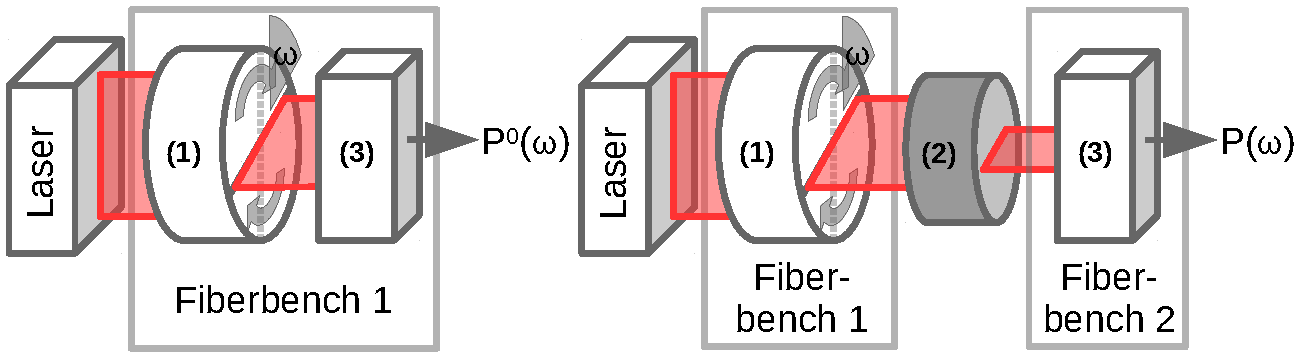
\includegraphics[width=\textwidth]{img/aufbau_faser_transmission.pdf}
                \caption[Transmissionsverhalten von optischen Fasern]{Der experimentelle Aufbau zur Bestimmung des Transmissionsverhaltens von optischen Fasern gegenüber linear polarisierter Strahlung. Die Polarisationsebene des Lasers wurde gedreht, indem die Halbwellenplatte (1) um beliebige Winkel $\omega$ rotiert wurde. Das Powermeter (3) maß die Leistung $P$ vor und hinter der optischen Faser (2).}
                \label{fig:method_transmissionFaser}
            \end{figure}
            
            Abbildung~\ref{fig:method_transmissionFaser} zeigt den Aufbau, der zur Bestimmung des Transmissionsverhaltens angewendet wurde. Für beliebige Rotationen der Halbwellenplatte \optelem{W1} wurde die Laserleistung direkt hinter der Halbwellenplatte und nach Passieren der Halbwellenplatte und der zu charakterisierenden optischen Faser gemessen. Es wurde festgehalten: Der Rotationswinkel von \optelem{W1} und die gemessenen Leistung vor und hinter der optischen Faser.
        
            \begin{figure}[!b]
                %
                %   MESSEN VON STOKES VEKTOREN AN FASERN
                %
                \centering
                \subfloat[]{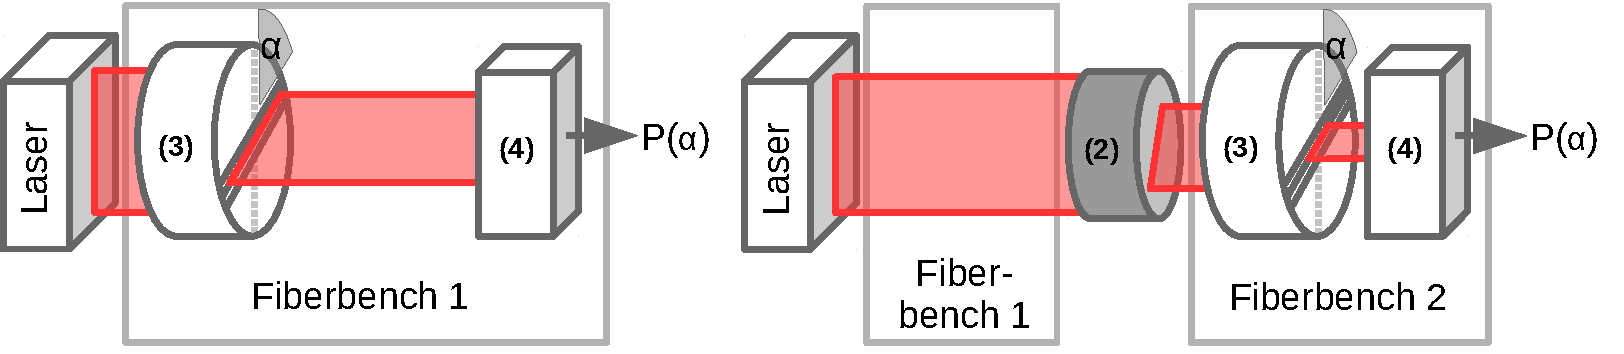
\includegraphics[width=\textwidth]{img/aufbau_faser_stokesvek_koord.pdf}\label{subfig:method_stokesFaser_koord}} \\
                \subfloat[]{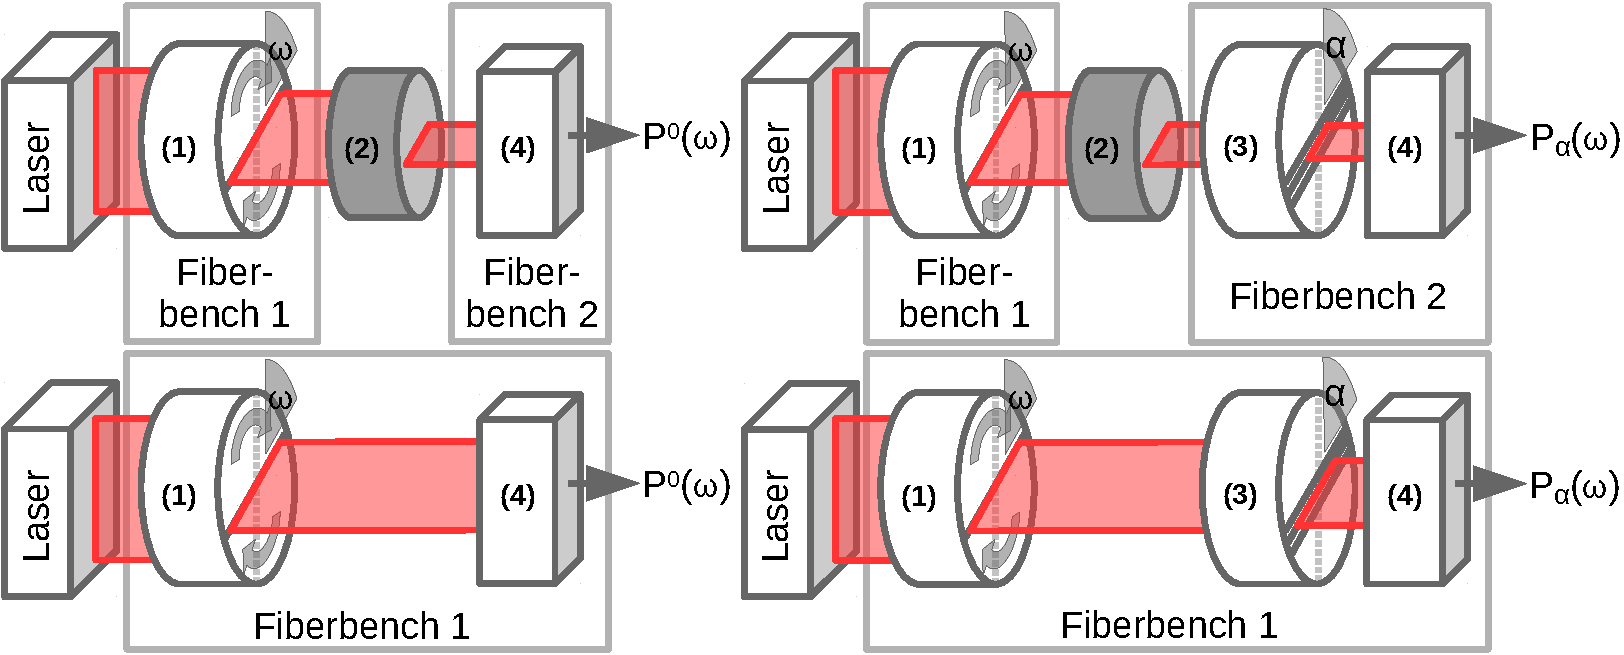
\includegraphics[width=\textwidth]{img/aufbau_faser_stokesvek.pdf}\label{subfig:method_stokesFaser_stokes}}
                \caption[Messen von Stokesparametern]{Der experimentelle Aufbau zum Ermitteln der ersten drei Stokesparameter vor und hinter einer optischen Faser. \subref{subfig:method_stokesFaser_koord}~Definition der Koordinatensysteme. Die Koordinatensysteme für die erste und zweite Fiberbench wurden so gewählt, dass eine Rotation des Linearpolarisators (3) um $\alpha = \{\SI{0}{\degree}, \SI{180}{\degree}\}$ die am Powermeter (4) messbare Laserleistung $P(\alpha)$ maximiert und eine Rotation um $\alpha = \SI{90}{\degree}$ sie minimiert.
                \subref{subfig:method_stokesFaser_stokes}~Messen der Stokesparameter. Der Stokesvektor der Strahlung wurde mit und ohne die optische Faser (2) bestimmt. Die Polarisationsebene des Lasers wurde mit der Halbwellenplatte (1) gedreht, indem (1) um beliebige Winkel $\omega$ gedreht wurde. Das Powermeter (4) maß die Leistung $P$ für verschiedene Rotationen des Linearpolarisators (3) um den Winkel $\alpha \in \{\SI{0}{\degree}, \SI{45}{\degree}, \SI{90}{\degree}, \SI{135}{\degree}\}$.}
                \label{fig:method_stokesFaser}
            \end{figure}
            
            Die ersten drei Komponenten des Stokesvektors, der die Polarisation einer Lichtwelle beschreibt, sind durch die vier Messwerte definiert, welche durch den Versuchsaufbau in Abbildung~\ref{subfig:method_stokesFaser_stokes} bestimmt wurden. Vor der Messung wurden für die Fiberbench vor der zu charakterisierenden Faser \optelem{B1} und der Fiberbench hinter der Faser \optelem{B2} ein Koordinatensystem definiert. Dafür wurde, wie Abbildung~\ref{subfig:method_stokesFaser_koord} zeigt, nur der Linearpolarisator \optelem{P3} und das Powermeter \optelem{PM} im Strahlengang platziert. Der Linearpolarisator wurde gegen den Uhrzeigersinn so gedreht, dass die gemessene Laserleistung maximal wurde. Der entsprechende Rotationswinkel wurde als $\alpha \coloneqq \SI{0}{\degree}$ definiert. Um sicher zu stellen, dass das Koordinatensystem richtig definiert war, wurde \optelem{P3} gegen den Uhrzeigersinn gedreht bis die von Powermeter registrierte Laserleistung minimal war. Dies sollte eine Rotation um \SI{90}{\degree} erfordern. Zuletzt wurde \optelem{P3} gegen den Uhrzeiger gedreht bis die Laserleistung wieder maximal wurde. Dies sollte ebenfalls eine Rotation um \SI{90}{\degree} erfordern. In allen durchgeführten Experimente erfüllten die definierten Koordinatensysteme diese Kriterien im Rahmen der Messungenauigkeit.
  
            \begin{figure}[!b]
                \center
                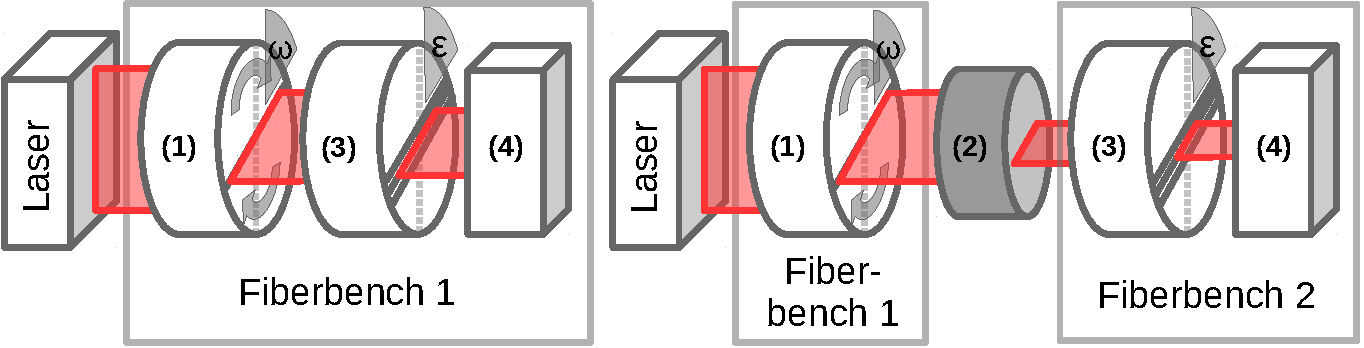
\includegraphics[width=\textwidth]{img/aufbau_faser_rotation.pdf}
                \caption[Rotation der Polarisationsebene durch optische Fasern]{Der experimentelle Aufbau zur Charakterisierung des Einflusses von optischen Fasern auf die Lage der Polarisationsebene von linear polarisierten Lichtwellen. Die Halbwellenplatte (1) wurde um beliebige Winkel $\omega$ rotiert, um die Polarisationsebene des Lasers zu drehen. Anschließend wurde mit Hilfe des Powermeters (4) der Linearpolarisator (3) um einen Winkel $\varepsilon$ rotiert, sodass (3) parallel zur Polarisationsebene der Strahlung stand. Die Messung erfolgte sowohl vor als auch hinter der charakterisierten Faser (2).}
                \label{fig:method_rotationFaser}
            \end{figure}
            
            Aufbau~\ref{subfig:method_stokesFaser_stokes} ermöglichte das Bestimmen der Stokesparameter. Für eine beliebige Rotationen der Halbwellenplatte \optelem{W1} wurden fünf Messungen sowohl vor als auch hinter der Faser vorgenommen. Zuerst wurde mit dem Powermeter \optelem{PM} die Laserleistung ohne den Linearpolarisator \optelem{P3} gemessen. Anschließend folgten vier Messungen mit \optelem{P3} rotiert um \SIlist{0; 45; 90; 135}{\degree}. \optelem{P3} wurde dabei direkt vor \optelem{PM} im Strahlengang platziert. Es wurden festgehalten: Die Position der Halbwellenplatte \optelem{W1}, die Leistung vor der Faser ohne \optelem{P3}, die Leistung hinter der Faser ohne \optelem{P3}, die Leistung vor der Faser für alle vier Rotationen von \optelem{P3} und die Leistung hinter der Faser für alle vier Rotationen von \optelem{P3}.
            
            In welchem Maße die optischen Fasern \optelem{F2} und \optelem{F3} die Polarisationsebene von linear polarisierter Strahlung rotieren, wurde mit Aufbau~\ref{fig:method_rotationFaser} ermittelt. Die Halbwellenplatte \optelem{W1} wurde vor der zu charakterisierenden optischen Faser im Strahlengang platziert. Der Linearpolarisator \optelem{P3} wurde vor das Powermeter im Strahlengang positioniert. \optelem{W1} wurde um beliebige Winkel gedreht und \optelem{P3} sowohl vor als auch hinter der Faser so gedreht, dass die vom Powermeter gemessene Leistung maximiert wurde. Es wurden festgehalten: Der Rotationswinkel der Halbwellenplatte \optelem{W1}, der Rotationswinkel des Linearpolarisators \optelem{P3} vor der optischen Faser und sein Rotationswinkel hinter der optischen Faser.
            
        
        \section{Polarisationsabhängige Messung von Spektren}\label{sec:appendix_method_spectra}
        
            Zur Charakterisierung des WiTecs wurden Spektren mit linear polarisiertem Weißlicht aufgenommen. Das Weißlicht wurde durch eine kalibrierte Weißlichtlampe des Typs HCA-5208 (Kaiser Optical Systems, Ann Arbor, Michigan, Vereinigte Staaten von Amerika) erzeugt. Die Messung erfolgte sowohl mit als auch ohne dem Mikroskop und der optischen Faser. Die Messung der Proben erfolgte ebenfalls polarisationsabhängig.
            
            \begin{figure}[!b]
                %
                %   FIG: AUFBAU WEIßLICHTSPEKTREN
                %
                \centering
                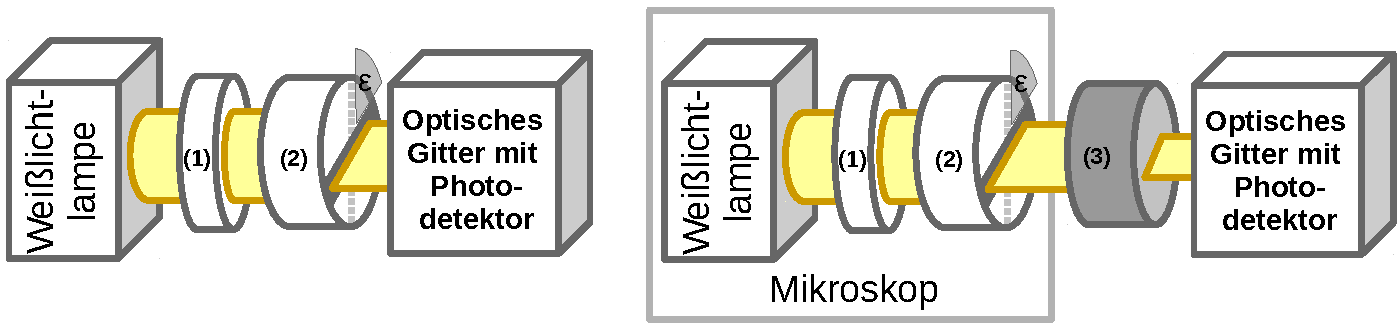
\includegraphics[width=\textwidth]{img/aufbau_weisslicht.pdf}
                \caption[Polarisationsabhängige Weißlichtspektren]{Der experimentelle Aufbau zum polarisationsahängigen Messen von Weißlichtspektren. Das Weißlicht wurde durch den Depolarisator (1) und den Linearpolarisator (2) entlang eines beliebigen Rotationswinkels $\varepsilon$ linear polarisiert. Die Einkopplung des Lichts erfolgte entweder durch das Ramanmikroskop und die Mehrmodenfaser \optelem{F3} (3) leitete die Lichtwelle zum Detektorsystem oder direkt am Detekor.}
                \label{fig:method_weisslicht}
            \end{figure}
            
            
            \begin{figure}[!b]
                %
                %   AUFBAU RAMANSPEKTREN
                %
                \centering
                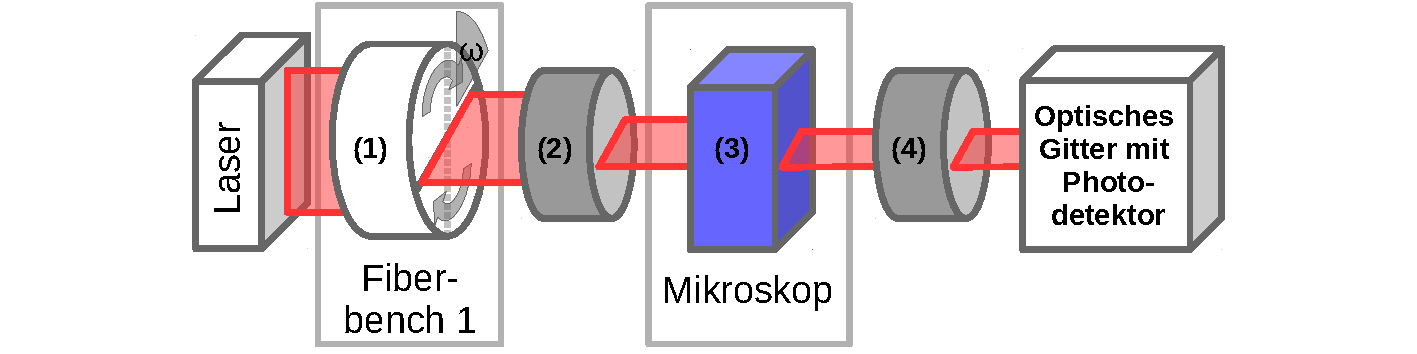
\includegraphics[width=\textwidth]{img/aufbau_ramanspektren.pdf}
                \caption[Polarisationsabhängige Ramanspektren]{Der experimentelle Aufbau zum polarisationsahängigen Messen von Ramanspektren am WiTec. Die Polarisationsebene des Laserstrahls wurde durch die Halbwellenplatte (1) beliebig rotiert, indem sie um den Winkel $\omega$ gedreht wurde. Die Einmodenfaser \optelem{F2} (2) leitete den Anregungslaser in das Ramanmikroskop mit der Probe (3). Das rückgestreute Licht wurde durch die Mehrmodenfaser \optelem{F3} (4) zum Photodetektorsystem geleitet.}
                \label{fig:method_ramanspektrum}
            \end{figure}
            
            
            Die Weißlichtspektren wurden mit dem Aufbau nach Abbildung~\ref{fig:method_weisslicht} gemessen. Das Licht der Weißlichtlampe wurde im Freespace durch den Depolarisator \optelem{DP} gestrahlt. Anschließend wurde es durch den Linearpolarisator \optelem{P3} linear polarisiert. Durch Rotation von \optelem{P3} wurde die Polarisationsebene der Strahlung eingestellt. Wenn die Einkopplung durch das Mikroskop erfolgte, wurde das Weißlicht durch die Mehrmodenfaser \optelem{F3} zum Detektor geleitet. Die Weißlichtspektren, welche ohne das Mikroskop gemessen wurden, wurden \SI{0,23}{\second} integriert und \num{20} Mal akkumuliert. Die Weißlichtspektren, welche mit dem Mikroskop gemessen wurden, wurden \SI{60}{\second} integriert und zwei Mal akkumuliert.
            
            Von Tetrachlormethan, Phenylalanin (\chemical{Phe}), 4-Acetaminophenol (\chemical{4-AAP}) und Trilaurinsäureglycerolester (Trilaurin) wurden Ramanspektren in Abhängigkeit der Polarisation des Anregungslasers aufgenommen. Die Chemikalien wurden von Sigma-Aldrich bezogen und ohne weitere Aufbereitung verwendet. Trilaurin wurde auf einer Heizplatte bei \SI{60}{\celsius} geschmolzen und in flüssigen Aggregatzustand ohne Küvette gemessen. Von \chemical{Phe} wurde eine gesättigte wässrige Lösung hergestellt, indem \chemical{Phe} in Salzsäure bei $\pH = 1$ gelöst wurde. Die Lösung wurde in einer Quarzküvette gemessen. \chemical{4-AAP} wurde fein zermahlen, anschließend verdichtet und als Feststoff gemessen. \ce{CCl4} wurde ohne weitere Probenvorbereitung in einer Quarzküvette gemessen.
            
            Die Aufnahme erfolgte mit dem Aufbau in Abbildung~\ref{fig:method_ramanspektrum}. Die Rotation der Halbwellenplatte \optelem{W1} beeinflusste die Lage der Polarisationsebene~\cite{gil_polarized_2016}, bevor der Anregungslaser durch die Einmodenfaser \optelem{F2} ins Mikroskop mit der vorbereiteten Probe geleitet wurde. Das rückgestreute Licht wurde in die Mehrmodenfaser \optelem{F3} eingekoppelt und zum Detektorsystem geführt. Für beliebige Positionen von \optelem{W1} wurden die Ramanspektren mit Integrationszeiten und Akkumulationen nach Tabelle~\ref{tab:method_ramanspektren} gemessen.
            
            \begin{table}[!h]
                %
                %   MESSBEDINGUNGEN RAMANSPEKTREN
                %
                \centering
                \caption[Messbedinungen der Ramanspektren]{Messbedingungen, Integrationszeit~$t$ und Zahl der Akkumulationen~$n$ der aufgenommenen Ramanspektren.}
                \label{tab:method_ramanspektren}
                \begin{tabular}{l l S[table-number-alignment = center] S[table-number-alignment = center]}
                    \toprule
                    Probe & Bedingungen & {$t / \si{\second}$} & {$n$} \\
                    \midrule
                    Tetrachlormethan   & flüssig                        & 45    & 6     \\
                    Phenylalanin       & gelöst ($\pH=1$)               & 600   & 1     \\
                    4-Acetaminophenol  & fest                           & 60    & 4     \\
                    Trilaurin          & flüssig (\SI{60}{\celsius})    & 60    & 10    \\
                    \bottomrule
                \end{tabular}
            \end{table}
            
        \section{Quantenchemische Berechnungen}
            %
            %   Wie werden Gaussian Berechnungen durchgeführt?
            %   Wie werden Raman Tensoren in Müllermatrizen übersetzt?
            %
            Die untersuchten Stoffe Tetrachlormethan, Phenylalanin, 4-Acetaminophenol und Trilaurin wurden mit \texttt{Gaussian16} quantenchemisch berechnet, um die experimentellen Daten mit Simulationen vergleichen zu können~\cite{frisch_gaussian_2016}. Alle Berechnungen wurden mittels Dichtefunktionaltheorie (DFT) und dem Funktional \texttt{B3LYP} durchgeführt. Zuerst wurden die Molekülgeometrie auf dem Basissatz \texttt{3-21G} voroptimiert. Anschließend folgte die Geometrieoptimierung und Frequenzrechnung mit dem Basissatz \texttt{6-31+G\te{*}}. Die Option \texttt{freq(raman, \linebreak printderivatives)} war aktiviert, damit die berechneten Ramantensoren in die .LOG-Datei geschrieben wurden.
            
            \texttt{PolaRam} wurde verwendet, um die Ramantensoren in den Müllerformalismus zu transformieren~\cite{eichhorn_polaram_2020}. Die Ramantensoren wurden mit \texttt{PolaRam}s \texttt{extract}-Befehl aus den Ausgabedatei von \texttt{Gaussian} gelesen und anschließend mit dem \texttt{convert}-Befehl in den Müllerformalismus übersetzt. Die Validierungsgrenze betrug zwei Nachkommastellen. Dass bedeutet \texttt{convert} iterierte die Monte-Carlo-Simulation bis der Depolarisationsgrad der Müllermatrix auf zwei Nachkommastellen dem Depolarisationsgrad des ursprünglichen Ramantensors übereinstimmte~\cite{eichhorn_polaram_2020, eichhorn_beschreibung_2020}. Das konnte \numrange{1000000}{10000000} Iterationen dauern.
\end{document}